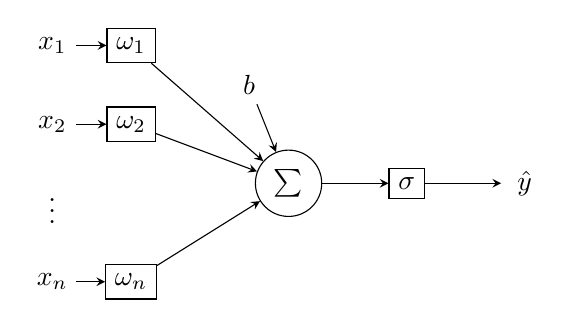
\begin{tikzpicture}[>=stealth, scale=1]

    % Define input nodes
    \node at (0, 1.5) {$x_1$};
    \node at (0, 0.5) {$x_2$};
    \node at (0, -0.5) {$\vdots$};
    \node at (0, -1.5) {$x_n$};

    % Define weight nodes
    \node[draw, rectangle] (w1) at (1, 1.5) {$\omega_1$};
    \node[draw, rectangle] (w2) at (1, 0.5) {$\omega_2$};
    \node[draw, rectangle] (wn) at (1, -1.5) {$\omega_n$};

    % Summation node
    \node[circle, draw] (sum) at (3, -0.25) {$\sum$};

    % Bias input
    \node at (2.5, 1.0) (b) {$b$};
    \draw[->] (b) -- (sum);

    % Sigma node
    \node[draw] (sigma) at (4.5, -0.25) {$\sigma$};

    % Output node
    \node at (6, -0.25) {$\hat{y}$};

    % Connect input to weights
    \draw[->] (0.3, 1.5) -- (w1);
    \draw[->] (0.3, 0.5) -- (w2);
    \draw[->] (0.3, -1.5) -- (wn);

    % Connect weights to summation node
    \draw[->] (w1) -- (sum);
    \draw[->] (w2) -- (sum);
    \draw[->] (wn) -- (sum);

    % Connect summation to sigma (activation function)
    \draw[->] (sum) -- (sigma);

    % Connect sigma to output
    \draw[->] (sigma) -- (5.7, -0.25);

\end{tikzpicture}